\documentclass[a4paper, 11pt]{report}

% Extra characters
\usepackage[utf8]{inputenc}

% Subfiles
\usepackage{subfiles}

% Document format
\usepackage[a4paper, left=2.5cm, right=2.5cm, top=2.5cm, bottom=2.5cm]{geometry}

% Line spacing
\usepackage[onehalfspacing]{setspace}

% Language used
\usepackage[portuguese]{babel}

% Font
\usepackage{helvet}
\renewcommand{\familydefault}{\sfdefault}

% Captions
\usepackage{caption}
\DeclareCaptionFormat{captionFormat}{\fontsize{9}{11}}
\captionsetup{format=captionFormat}

% Figures
\usepackage{graphicx}
\usepackage{wrapfig}

% Tables
\usepackage{booktabs}
\usepackage{array}

% Improve justification document wide
\usepackage{microtype}

% Compact lists
\usepackage{enumitem}
 
% Customize the page layout of your LaTeX documents
\usepackage{fancyhdr}

% Paragraph indentation
\usepackage{indentfirst}
% Set the indentation length
\setlength\parindent{1.25cm}

% Glossary and acronyms
\usepackage[acronym, nogroupskip, toc]{glossaries}

% Bibliography
% \usepackage{biblatex}
% \addbibresource{references.bib}

% Appendices
\usepackage[toc,page]{appendix}

% Document bookmarks
\usepackage{pdfpages}
\usepackage[
	linktocpage=true,
	colorlinks=true,
	allcolors=cyan,
	bookmarks=true,
	bookmarksopen=true,
	bookmarksnumbered=true,
	pdfpagelabels=true
]{hyperref}
\usepackage{bookmark}

% Mini TOC in each chapter
\usepackage{minitoc}
% Silence minitoc warnings
\usepackage{silence}
\WarningFilter{minitoc(hints)}{W0023}
\WarningFilter{minitoc(hints)}{W0024}
\WarningFilter{minitoc(hints)}{W0028}
\WarningFilter{minitoc(hints)}{W0030}

% Set the number of depth of sections
\setcounter{secnumdepth}{5}
\setcounter{tocdepth}{5}
\setcounter{minitocdepth}{5}

\glsdisablehyper
\makenoidxglossaries
\newacronym{arima}{ARIMA}{\gls{autoregressive integrated moving average}}

\newacronym{ia}{IA}{\gls{inteligencia artificial}}

\newacronym{ml}{ML}{\gls{machine learning}}
% \gls - lowercase singular
% \Gls - uppercase singular
% \glspl - lowercase plural
% \Glspl - uppercase plural

\newglossaryentry{git}
{
	name=Git,
	description={Distributed version-control system for tracking changes in source code
	during software development}
}


\begin{document}

% \setcounter{page}{0}
\pagenumbering{gobble}

% Cover
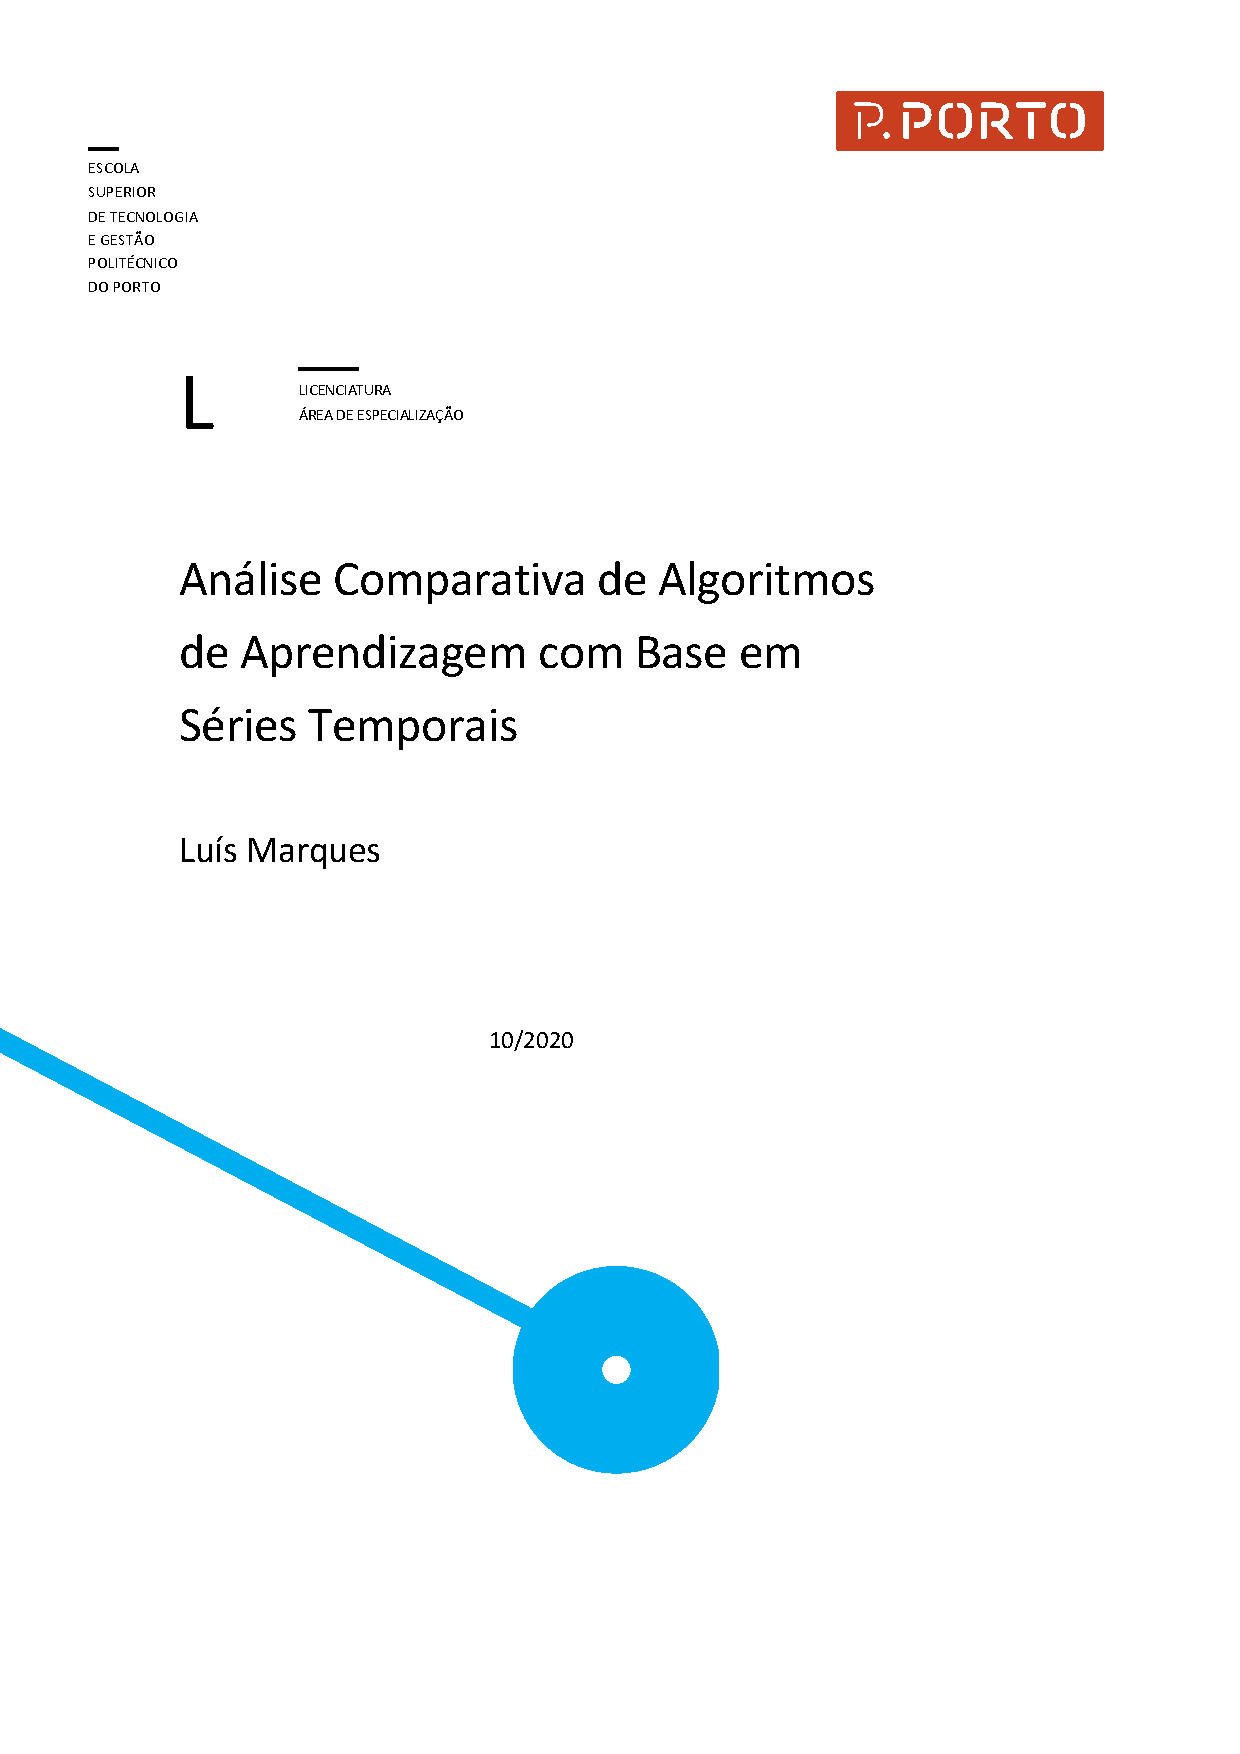
\includepdf{../private_assets/Cover.pdf}

% Blank page
\subfile{blank_page.tex}

% Back cover
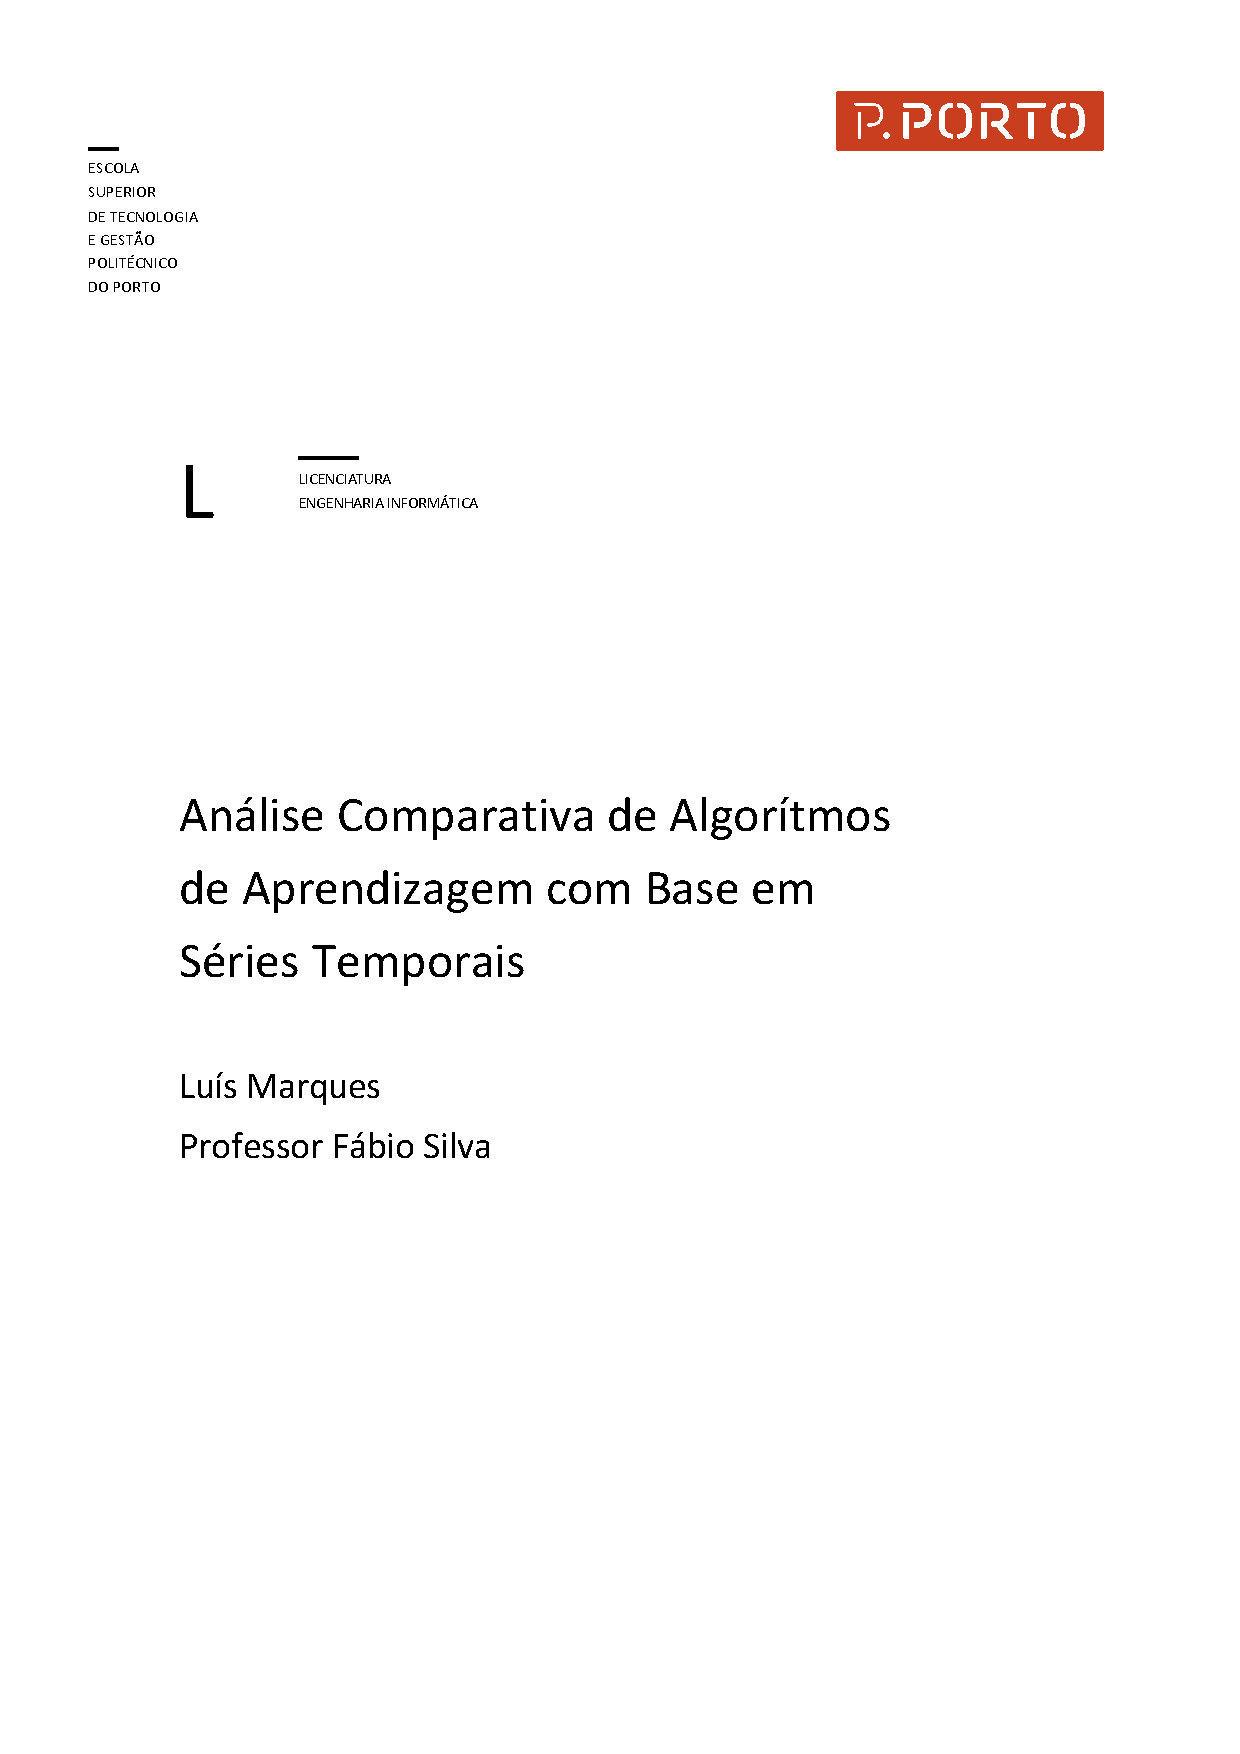
\includepdf{../private_assets/BackCover.pdf}

% Blank page
\subfile{blank_page.tex}

\pagestyle{fancy}
\fancyhf{}
\renewcommand{\headrulewidth}{0pt}
\fancyfoot[R]{\thepage}
\pagenumbering{roman}

% Author's Biography
\subfile{author_biography.tex}

% Blank page
\subfile{blank_page.tex}

% Abstract
\subfile{abstract.tex}

% Blank page
\subfile{blank_page.tex}

% Initialization of minitoc
\dominitoc
\mtcsettitle{minitoc}{}
\mtcsetoffset{minitoc}{-1.0em}
\renewcommand{\mtifont}{\large\sffamily}
\renewcommand{\mtcfont}{\small\sffamily}
\renewcommand{\mtcSfont}{\small\sffamily}
\renewcommand{\mtcSSfont}{\small\sffamily}
\renewcommand{\mtcSSSfont}{\small\sffamily}

% Table of contents
\tableofcontents
\newpage

% Blank page
\subfile{blank_page.tex}

% List of figures
\listoffigures
\newpage

% Blank page
\subfile{blank_page.tex}

% Glossary
\printnoidxglossary
\adjustmtc
\newpage

% Blank page
\subfile{blank_page.tex}

% Abbreviations
\printnoidxglossary[type=\acronymtype, title={Abreviaturas}]
\adjustmtc
\newpage

% Blank page
\subfile{blank_page.tex}

\pagenumbering{arabic}

% Chapter 1
\subfile{chapt_1.tex}

% Chapter 2
\subfile{chapt_2.tex}

% Chapter 3
\subfile{chapt_3.tex}

% Chapter 4
\subfile{chapt_4.tex}

% Chapter 5
\subfile{chapt_5.tex}

% Blank page
\subfile{blank_page.tex}

% References
\subfile{libs/references.tex}
% \chapter*{References}
% \printbibliography[title={References}]
% \newpage

% Blank page
% \subfile{blank_page.tex}

% Appendices
% \subfile{appendices.tex}

\end{document}